\indent\textbf{\emph{Paradigm shift in computing.}}
In the last decade, we witnessed a growing demand to perform large-scale
computations, such as protein folding, fluid dynamics, weather prediction and
wide range of optimization for military and industry.
The scale of such computations exceedes abilities of a single computer, hence computations are performed on large sets of machines that cooperate over interconnecting network, collectively called the \emph{computer cluster}.
Owning and maintaing such infrastructure is often impractical and expensive, and parties look for alternative ways to perform computations.
Outsourcing such computations provides a wide range of benefits.
First of all, it mitigates the costs of infrastructure management and maintenance.
This is crucial especially for computational tasks that arise occasionally, such as optimizations for industries \maciek{More examples needed. Those listed before are naive to list as occasional}.
In addition, it dismisses the need to foresee the appropriate demand for resources.
If the demand for resources increases unexpectedly, it can be immediately provided without physical extension of the infrastructure.
Above rationalities combined led to shift the computations to large, dedicated and remote computer clusters that are called \emph{data centers}, and coined the term \emph{cloud computing}.\maciek{the last ``and'' would need parethesis}

The demand for outsourcing computations to the cloud created a whole market for such services.
Modern general-purpose and open for general use data centers such as Microsoft Azure \cite{url-azure}, Amazon Elastic Cloud Computing EC2 \cite{url-amazon-ec2} or Google Compute Engine \cite{url-gce} provide convenient on-demand computational power while hiding most of details concerning resource management.

Computational tasks require multiple types of resources to complete: CPU time, memory, I/O operations and network bandwith.
Demand for resources often vary in time and is unpredictable or expensive to predict.
For this reason, the data center that performs \emph{just one task at the time} are doomed to waste resources.
However, co-existence of multiple tasks in the data center allows to compensate for the variable demand for resources of computational tasks by resource-aware scheduling.
Such techniques are especially useful in (but not limited to) computationally-intensive applications, where the response time is not the primary concern.

\emph{From the perspective of an data center owner}, the main goal 
is an efficient management of resources. This is interwined with 
a multitude of problems and requirements: security in resource-sharing scenarios,
standarization and compatibility, automation, availability, extensibility and
modularity, recovery, and many more. An important class of new challenges in
data center is \emph{optimization of resource usage}. In particular, 
processing speed can
scale down to save energy, memory can be shared or distributed, and cooperating
processes can migrate closer in the network to save bandwidth.

\section{Machine virtualization}

This computational paradigm shift is strongly connected with the advancements 
in the underlying computational infrastructure, both in hardware and in software. 
The processing capabilities of data centers 
would not be possible without improvements in
task isolation, resource sharing and transparent concurrency.
The software advancements played the
primal role in allowing data centers to grow without wasting its resources.

A particular piece of technology that suits the model of modern data center extraordinarly well is virtualization.
Virtualization provides an abstraction layer for the underlying hardware of a computer system, called the \emph{virtual machine}.
Virtual machine mimics functionality of the physical hardware so closely and
directly that it can be used as an environment for a complete operating system.
Such operating system, running on a virtual machine is called the \emph{guest
operating system}. It operates in additon to the \emph{host operating
system}, which operates directly on the physical hardware. 

Mature virtualization solutions are available for data center usage: Xen
\cite{url-xen}, KVM \cite{url-kvm}, Hyper-V \cite{url-hyperv}, VMware ESXi
\cite{url-vmware}. The perspective of the guest
operating system is restricted to such exposed virtual machine and is provided
with an illusion of possesing the whole computer system. The main features of
virtualization in datacenter is \emph{to provide the complete and
non-restricted environment} for the client that is isolated from the management
software and other clients' tasks.

Besides providing an abstraction layer, virtualization provides several
control features. Absolute control over the underlying, virtual hardware of
the guest operating system allows to suspend and resume the execution of the
guest operating system at will. Such functionality provides building blocks
for the feature of migration, which transfers the complete virtual machine to
a different physical machine. Possibility of migration plays an important role
in load balancing in the data center and allows for sophisticated
optimizations such as reducing network distance between communicating virtual
machines.

Data center consists of multiple virtual machines running on physical nodes
that are connected by physical network. Single virtual machine often provides
insufficient resources for the client, as its resources are limited by resources
available to its host. Data centers provide its resources to clients as a set
of virtual machines connected by a network. The network that connects virtual
machines is restricted and controlled in similar manner to hardware
virtualization, and is called a \emph{virtual network}. Cooperating virtual
machines are often refered to as a \emph{nodes} of a virtual network. To
guarantee certain quality of service (\emph{QoS}), up-front bandwidth
reservations are a requisite. However, the generality of performed calculations
results in unpredictibility of communication patterns and poses a challenge in
optimization of bandwidth reservations.

Virtualization allows
flexibility in renting infrastructure, and might offer savings in resource
management. However, efficient use of resources requires sophisticated
techniques to achieve its goal. In this thesis, we focus on using the tools
provided by modern virtualization techologies for efficient usage of important
resource in the data center -- the network bandwidth. Problem central to this
thesis is stated as follows:

\begin{center}
  \emph{How to assign virtual machines to physical machines to optimize network
  usage?}
\end{center}

We elaborate more in subsequent subsection.

\section{Algorithmic aspects of the virtual machines embedding}

To state optimization problems, we model certain aspects of data center operation.
Physical components of a data center are often modelled in form of a graph called a \emph{substrate network}, in which vertices correspond to \emph{physical machines}, and edges correspond to \emph{network interconnect}.
Communication cost between pair of physical machines is proportional to edge-distance in substrate network (the number of \emph{hops} in the substrate network).
Communication pattern among virtual machines is also modelled as a graph, called a \emph{communication graph}.
In such settings, the communication among virtual machines running on certain physical machines is modelled as a \emph{graph embedding} of communication graph into a substrate network.
In optimization of network usage, the objective function is the total cost of such embedding, measured in size of multiset of used edges of the host graph.

In this thesis we consider substrate networks in form of a tree, which models closely the popular topology of a Fat-Tree, but fails to approximate some sophisticated topologies such as a Butterfly Topology.
In the tree topology, we distinguish a specific class of physical machines that cannot host virtual machines, and their sole role is to transmit communication patterns.
Machines that are able to host virtual machines are placed in leaves of the substrate graph.


\begin{figure}[t]
\centering
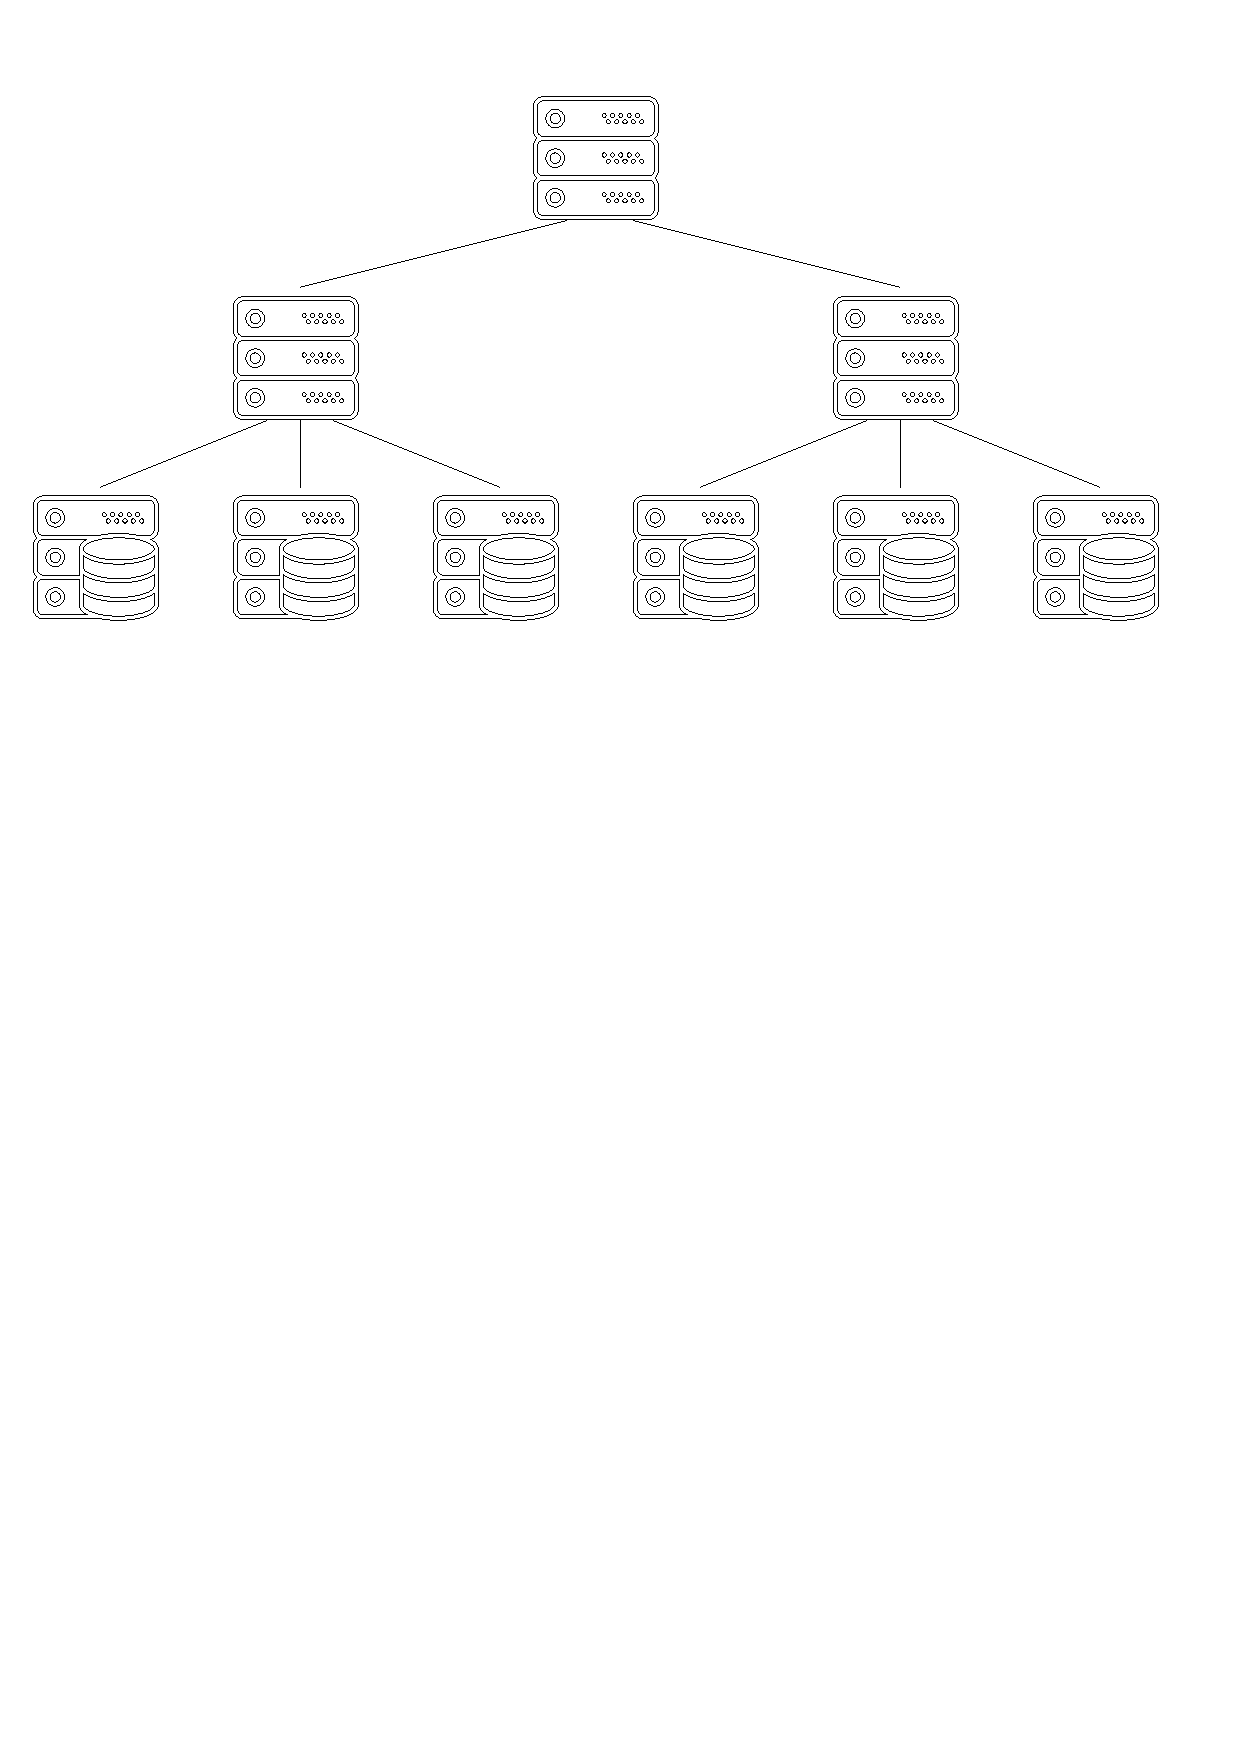
\includegraphics[width=0.79\columnwidth]{figs/tree-topology.pdf}
\caption{The model of typical data center.}\label{fig:overview}
\vspace{-1em}
\end{figure}

\section{Algorithmics aspects of network optimization}

TODO Tree Caching

\section{Contributions of this thesis and thesis organization}

In this thesis we consider two scenarios regarding virtual machines embeddings:
\begin{enumerate}
  \item The communication pattern among virtual machines is known up-front
  \item The communication pattern is not known, and has to be discovered and is a subject to changes over time
\end{enumerate}

\maciek{I realised that the paragraph below is wrong. In both cases the communication pattern is not known. The difference lies in how we proceed: either we try to discover patters, or we make complete graph reservations}

Consider the scenario, where the communication pattern is not known.
In order to guarantee certain quality of service (\emph{QoS}), we need to acquire network reservations for \emph{all} possible communication patterns among cooperating virtual machines.
Hence, in such scenario, we consider the worst-case communication graph in form of a clique.
The combinatorial problem that we consider in Part 1 is essentially the minimum-cost embedding of a clique in a tree, enriched by certain extensions motivated by Map-Reduce applications.
We consider the wide range of possible extensions, most notably:

\begin{itemize}
\item \emph{Data chunk processing}. In Map-Reduce applications, set of virtual machines processes large amounts of data that are stored in distributed file system. Each chunk of data must be assigned and transferred to a virtual machine. Data chunk transfer requires its own network reservations.

\item \emph{Data chunk replication}. Distributed file systems often store redundant copies of data chunks, called \emph{chunk replicas}. Only one copy of each data chunk replica must be processed, and we are free to choose the replica based on its placement.

\item \emph{Bandwidth constraints}. Each link in substrate network has its capacity. For the embedding to be feasible, the total network reservations has to obey link capacities.
\end{itemize}

Consider the scenario, where the communication pattern is not known.
Migration.



\subsection{Contributions on static mapping}

This paper initiates the formal study of data-locality and replica aware virtual network embedding problems in datacenters.
In particular, we decompose the general optimization problem into its fundamental aspects, such as
assignment of chunks, replica selection, and flexible virtual machine
placement, and answer questions such as:
\begin{enumerate}
\item Which chunks to assign to which virtual machine?

\item How to exploit redundancy and select good replicas?

\item How to efficiently embed virtual machines and their inter-connecting network?

\item Can the chunk assignment, replica selection and virtual machine embedding problems be jointly optimized, in polynomial time?
\end{enumerate}

We draw a complete picture of the problem space: We show that
even problem variants exhibiting multiple degrees of freedom in terms of
replica selection and embedding,
can be solved optimally in polynomial time, and we present several efficient
algorithms accordingly. However, we also prove limitations in terms of
computational tractability, by providing reductions from 3-D matching
and Boolean satisfiability ($\SAT$). Interestingly,
while it is well-known that (unsplittable) multi-commodity flow
problems are NP-hard in capacitated networks, our hardness results also hold in \emph{uncapacitated}
networks; moreover, we show that NP-hard problems already arise in small-diameter networks (as they are
widely used today~\cite{fattree}).

\subsection{Contribution on dynamic mapping}


This paper introduces the online Balanced RePartitioning problem (BRP),
a fundamental \emph{dynamic} variant of the classic graph clustering problem. 
We show that BRP features some interesting connections to other well-known
online graph problems. For $\ell=2$, BRP is able to simulate online paging problem
and for for $k=2$, BRP is a~novel online version of maximum matching.
We consider deterministic algorithms and make the following technical
contributions:

\begin{description}

\item[Algorithms for General Variant:]
For the non-augmented variant, in \ref{sec:upper}, we first present a~simple
$O(k^2 \cdot \ell^2)$-competitive algorithm. Our main technical contribution
is an $O((1+1/\eps) \cdot k \log{k})$-competitive deterministic algorithm
$\CREP$ for a setting with $(2+\eps)$-augmentation (\ref{sec:crep}).
We emphasize that this bound does not depend on~$\ell$. This is interesting,
as in many application domains of this problem, $k$ is small: for example, in
our motivating virtual machine collocation problem, a server typically hosts
only a small number of virtual machines (e.g., related to the constant number
of cores on the server).

\item[Algorithms for Online Rematching:]
For the special case of online rematching ($k=2$, but arbitrary~$\ell$), in
\ref{sec:k-two}, we prove that a variant of a greedy algorithm is
7-competitive. We also demonstrate a lower bound of 3 for any deterministic
algorithm.

\item[Lower Bounds:]
By a reduction to online paging, in \ref{sec:paging}, we show that
for two clusters no deterministic algorithm can obtain a better bound than
$k-1$. While this shows an~interesting link between BRP and paging, in
\ref{sec:lower-bounds}, we present a stronger bound. Namely, we
show that for $\ell \geq 2$ clusters, no deterministic algorithm can beat the
bound of $k$ even with an~arbitrary amount of augmentation, as~long~as~the
algorithm cannot keep all nodes in a~single cluster. In contrast, online
paging is known to~become constant-competitive with constant
augmentation~\cite{SleTar85}.

\end{description}




\subsection{Contributions on memory management in network devices}

\todo{Mixed with organization of the paper}

We initiate the study of a natural new caching with bypassing problem which
allows to account for tree-dependencies among items. The problem finds
immediate applications, e.g., in IP routing and software-defined networking
(see \lref[Section]{sec:motivation}).

In particular, we consider the online tree caching problem within the resource
augmentation paradigm: we assume that cache sizes of the online algorithm
($\kALG$)  and the optimal offline algorithm ($\kOPT$) may differ. We assume
$\kALG \geq \kOPT$ and let $R = \kALG/(\kALG-\kOPT+1)$.

In \lref[Section]{sec:algo}, we present an elegant deterministic online
algorithm~\ALG for this problem. While our algorithm is simple, its analysis
presented in \lref[Section]{sec:analysis} requires several non-trivial
insights into the problem. In particular, we rigorously prove that \ALG is
$O(h(T) \cdot R)$-competitive, where $h(T)$ is the height of tree~$T$. That
is, we show that there exists a constant~$\beta$, such that $\ALG(I) \leq
O(h(T) \cdot R) \cdot \OPT(I) + \beta$ for any input $I$. Note that this
result is optimal up to the factor~$O(h(T))$: in
\lref[Appendix]{sec:lower-bound-on-the-problem}, we show that the lower
bound~$R$ for the paging problem~\cite{competitive-analysis} implies an
$\Omega(R)$ lower bound for our problem for any $\alpha \geq 1$. Finally, in
\lref[Section]{sec:implementing_counters}, we show that \ALG can be
implemented efficiently.



\subsection{Performance metrics}

Methods of Measuring the Quality of Results

\subsubsection{Online Algorithms and Competitive Analysis}

Sleator, Tarjan: list update \cite{competitive-analysis}
Borodin book \cite{borodin-book}

\subsubsection{Time and Space Complexity and NP-completeness}


\section{Related Work}

\todo{Megre}

\subsection{Related Work on Static Mapping}


There has recently been much interest in programming models and distributed
system architectures for the processing and analysis of big data (e.g.~\cite{nodb,mapreduce,shark}). The model studied in
this paper is motivated by MapReduce~\cite{mapreduce} like batch-processing applications, also known
from the popular open-source implementation \emph{Apache Hadoop}.
These applications
generate large amounts of network traffic~\cite{orchestra,talk-about,amazonbw},
and over the last years, several systems have been proposed which provide
a provable network performance, also in shared cloud environments, by supporting
relative~\cite{faircloud,elasticswitch,seawall}
or, as in the case of our paper, \emph{absolute}~\cite{oktopus,secondnet,drl,gatekeeper,proteus} bandwidth reservations
between the virtual machines.

The most popular virtual network abstraction for batch-processing applications today is the \emph{virtual cluster},
introduced in the Oktopus paper~\cite{oktopus}, and later studied by many others~\cite{talk-about,infocom16,ccr15emb,proteus}. In particular, Proteus \cite{proteus} improves
upon the Oktopus~\cite{oktopus} embedding algorithm of fat-trees and makes the case
for a time-adaptive embedding. The Kraken system~\cite{infocom16} is based on an optimal
embedding algorithm of fat-trees and and allows to elastically scale both link as well as
node resources. In~\cite{ccr15emb}, Rost et al.~show that the virtual cluster abstraction
can even be embedded on general graphs in polynomial time, and initiate the algorithmic study
of a Hose interpretation of the virtual cluster abstraction.

Several heuristics have been developed to compute ``good'' embeddings of virtual clusters: embeddings
with small footprints (minimal bandwidth reservation costs).
The virtual network embedding problem has also been studied for more general graph abstractions
(e.g., motivated by wide-area networks).~\cite{boutaba-survey,fischer-survey}


From a theoretical perspective, the virtual network embedding problem can be seen as a generalization
of classic VPN graph embedding problems~\cite{Goyal2008,gupta2001provisioning},
in the sense that in virtual network embedding problems, also the embedding endpoints are flexible. In this respect, the virtual network embedding problem can also be seen as a generalization of the
classic NP-hard Minimum Linear Arrangement problem which asks for the
embedding of guest graphs on a simple \emph{line topology} (rather than tree-like topologies as
studied in this paper)~\cite{mla,mla-survey}.

However, to the best of our knowledge, we are the first to provide an algorithmic
study of the virtual cluster embedding problem which takes into account
data locality as well as the possibility to select replicas---aspects which so far have only
been studied from a best-effort perspective and using coarse-grained metrics (e.g., same rack or same server), thus limiting the flexibility of the
system~\cite{local-schedule-1,local-schedule-2,local-schedule-3}.

\noindent \textbf{Bibliographic Note.} A preliminary version of this paper appeared
at the 23rd IEEE International Conference on Network Protocols (ICNP), 2015~\cite{icnp15loc}.



\subsection{Related Work on Dynamic Mapping}


The static offline version of our problem, i.e., a problem variant where
migration is not allowed, where all requests are known in advance, and where
the goal is to find best node assignment to $\ell$ clusters, is known as the
$\ell$-balanced graph partitioning problem. The problem is 
NP-complete, and cannot even be approximated within any finite factor unless P
= NP~\cite{AndRae06}. The static variant where $n/\ell = 2$ corresponds to a
maximum matching problem, which is polynomial-time solvable. The static
variant where $\ell = 2$ corresponds to the minimum bisection problem, which
is already NP-hard~\cite{GaJoSt76}. Its approximation was studied in a long
line of work~\cite{SarVaz95,ArKaKa99,FeKrNi00,FeiKra02,KraFei06,Raec08} and
the currently best approximation ratio of $O(\log n)$ was given by
R{\"{a}}cke~\cite{Raec08}. The $O(\log^{3/2} n)$-approximation given by
Krauthgamer and Feige~\cite{KraFei06} can be extended to~general $\ell$, but
the running time becomes exponential in~$\ell$.

The inaproximability of the static variant for general values of $\ell$
motivated research on the bicriteria variant, which can be seen as the offline
counterpart of our cluster-size augmentation approach. Here, the~goal
is~to~develop $(\ell,\delta)$-balanced graph partitioning, where the graph has
to be partitioned into $\ell$ components of~size less than $\delta \cdot (n /
\ell)$ and the cost of the cut is compared to the optimal (non-augmented)
solution where all components are of size $n / \ell$. The variant where
$\delta \geq 2$ was considered in
\cite{LeMaTr90,SimTen97,EvNaRS00,EvNaRS99,KrNaSc09}. So far the best result is
an $O(\!\sqrt{\log n \cdot \log \ell})$-approximation by Krauthgamer et
al.~\cite{KrNaSc09}, which builds on ideas from the $O(\!\sqrt{\log
n})$-approximation algorithm for balanced cuts by Arora et al.~\cite{ArRaVa09}.
For smaller values of $\delta$, i.e., when $\delta = 1 + \eps$ with a fixed
$\eps > 0$, Andreev and R{\"{a}}cke gave an $O(\log^{1.5} n / \eps^2)$
approximation~\cite{AndRae06}, which was later improved to $O(\log n)$ by
Feldmann and Foschini ~\cite{FelFos15}.

The BRP problem considered in this paper was not previously studied. However,
it bears some resemblance to the classic online problems; below we highlight
some of them.

Our model is related to online
paging~\cite{SleTar85,FKLMSY91,McGSle91,AcChNo00}, sometimes also referred to
as online caching, where requests for data items (nodes) arrive over time and
need to be served from a cache of finite capacity, and where the number of
cache misses must be minimized. Classic problem variants usually boil down to
finding a smart eviction strategy, such as Least Recently Used (LRU). In our
setting, requests can be served remotely (i.e., without fetching the
corresponding nodes to a single cluster). In this light, our model is more
reminiscent of caching models \emph{with
bypassing}~\cite{EpImLN11,EpImLN15,Irani02}. Nonetheless, we show that BRP is
capable of emulating online paging.

The BRP problem is an example of a non-uniform problem~\cite{KaMaMO94}: the
cost of changing the state is higher than the cost of serving a single
request. This requires finding a~good trade-off between serving requests
remotely (at a low but repeated communication cost) or migrating nodes into a
single cluster (entailing a potentially high one-time cost). Many
online problems exhibit this so called \emph{rent-or-buy} property, e.g., ski
rental problem~\cite{KaMaMO94,LoPaRa08}, relaxed metrical task
systems~\cite{BaChIn01}, file migration~\cite{BaChIn01,BiByMu17}, distributed
data management~\cite{BaFiRa95,AwBaFi93,AwBaFi98}, or rent-or-buy network
design~\cite{AwAzBa04,Umboh15,FeWiLe16}.

There are two major differences between BRP and the problems listed above.
First, these problems typically maintain some configuration of servers or
bought infrastructure and upon a new request (whose cost typically depends on
the distance to the infrastructure), decide about its reconfiguration (e.g.,
server movement or purchasing additional links). In contrast, in our model,
\emph{both} end-points of a communication request are subject to optimization.
Second, in the BRP problem a request reveals only very limited information
about the optimal configuration to serve it: There exist relatively long
sequences of requests that can be served with zero cost from a fixed
configuration. Not only can the set of such configurations be very large, but
such configurations may also differ significantly from each other.

\subsection{Related Work on Caching / Cache Management / Resource Management}

Our formal model is a novel variant of competitive paging, a~classic online
problem. In the framework of the competitive analysis, the paging problem was
first analyzed  by Sleator and Tarjan~\cite{competitive-analysis}, who showed
that algorithms \textsc{Least-Recently-Used}, \textsc{First-In-First-Out} and
\textsc{Flush-When-Full} are $\kALG / (\kALG - \kOPT + 1)$-competitive 
and no deterministic algorithm can beat this ratio. In the non-augmented case
when $\kALG = \kOPT = k$, the competitive ratio is simply $k$.

The simple paging problem was later generalized to allow different fetching
costs (weighted paging)~\cite{double-coverage,young-paging-greedy-dual} and
additionally different item sizes (file caching)~\cite{young-paging-landlord},
with the same competitive ratio. Asymptotically same results can be achieved
when bypassing is allowed (see \cite{caching-rejection-penalties,paging-irani}
and references therein). With randomization, the competitive ratio can be
reduced to $O(\log k)$ even for file caching~\cite{generalized-caching-optimal}. 
The lower bound for randomized algorithms is $H_k = 
\Theta(\log k)$~\cite{paging-mark} and is matched by known paging
algorithms~\cite{paging-optimal-easy,paging-optimal-difficult}.

To the best of our knowledge, the variant of caching, where fetching items to
the cache is not allowed unless some other items are cached (e.g., because of 
tree dependencies) was 
not considered previously in the framework of competitive analysis. Note that
there is a seemingly related problem called restricted
caching~\cite{restricted-caching} (there are also its variants called matroid
caching~\cite{matroid-caching} or companion caching~\cite{companion-caching}).
Despite naming similarities, the restricted caching model is completely
different from ours: there the restriction is that each item can be placed only in
a~restricted set of cache locations.





\section{Bibliographic notes}

Parts of this thesis were co-published by the author of this thesis in the following conferences and journals: ICNP TODOCITE, ACM SPAA TODOCITE, DISC TODOCITE and Journal of Theoretical Computer Science TODOCITE.
In addition, parts of this thesis were published in Alexandra Spyra's master thesis and Carlo Fuerst's doctorial thesis.